\documentclass{article}
%\documentclass[twocolumn]{article}
\usepackage{fullpage}
\usepackage{amsmath}
\usepackage{apacite}
\usepackage{url}
\usepackage{graphicx}
\usepackage{subfigure}
\usepackage{color}
\usepackage{colortbl}
\usepackage{tabularx}
%\usepackage{paralist}
%\usepackage{mdwlist}
\newcommand{\comment}[1]{}

\usepackage{float}
\newfloat{Algorithm}{h!}{}{}

% program-related commands
\usepackage{program}
\renewcommand{\|}{\origbar} % use this instead of '|' because program package redefines '|'
\renewcommand{\WHILE}{\mbox{{\bf while} }\tab}
\renewcommand{\FOR}{\mbox{{\bf for} }\tab}
\renewcommand{\IF}{\mbox{{\bf if} }\tab}
\newcommand{\IN}{\mbox{ {\bf in} }}

\newcommand{\xyspace}{{\em xy} space}

\begin{document}
\title{Object Detection with AGiNG}
\author{Andrew Stromme \& Ryan Carlson}
\date{May 14, 2010}
\maketitle

\begin{abstract}
  In this paper we present a modification to the Growing Neural Gas (GNG) algorithm called {\em Aging Growing Neural Gas} (AGiNG) specifically tuned for object detection and tracking. We propose that this GNG can be used as a replacement for the `blobify' filter found in Pyro libraries\footnote{\url{http://pyrorobotics.org/?page=Pyro}} since our GNG can track multiple objects of the same color as they move through a scene. We note that, contrary to many other object tracking methods, we do not use edge detection but are still able to produce encouraging results.
  
  The normal GNG algorithm uses a space-filling graph to categorize a domain. Each edge has an age that is reset based on how accurately the graph is categorizing the space. Our implementation adds a {\em total age} to the GNG that gives us extra context about how long edges have existed and allows us to dismiss younger ages if necessary. We have also added a host of image-specific features to optimize the GNG for our purposes. Once we have correctly categorized the scene we can identify objects and track them as they move through the scene using efficient graph traversal algorithms. We have tested our implementation on static and moving images, both computer-generated and real life. Additionally, we have had some success with identifying and tracking images with a webcam and have interfaced with a Sony AIBO to have it move appropriately to given input.
\end{abstract}

\section{Introduction}

%Talk about using a modified Growing Neural Gas to track objects. Why is this cool? $-->$ Don't need any type of edge detection. Computationally inexpensive (amortized). We see this as a replacement for the 'blobify' filter.

%We want to create a Growing Neural Gas that can identify objects and then have the AIBO track it. Talk about limitations of blobify and how this improves it.

Our task is object recognition and tracking using Aging Growing Neural Gas (AGiNG), a modified Growing Neural Gas. We provide an image for the GNG to categorize, and the GNG identifies the objects. In the case of a movie, the GNG must be able to update and adapt to the scene. Objects moving across a canvas need to be identified from one frame to another. To test the algorithm's capacity for tracking, we used sets of simple, computer-generated images along with real-world images taken with a camera. Additionally, we created computer-generated sequences of images that served as a simple movie. On the other end, we ran the GNG on real-time input coming from a webcam and got encouraging results. We also interfaced with the AIBO and were able to give it appropriate commands given an object to follow moving the scene.

The graph is initially somewhat expensive to build, taking on average about 10,000 steps to categorize a scene. After that point, however, the cost becomes much less. The GNG has an implicit memory of the scene that we use to our advantage. As objects move around -- as the scene changes -- the graph must only undergo small, local changes to accurately classify the scene. Contrast this with other object detection algorithms that must, at each change, reevaluate the entire space. Moreover, on a consumer-level laptop the initial categorization stage takes less than one second. 

Our object detection is based around the color of and distance between two pixels. We see the AGiNG as a replacement of the `blobify' filter from Pyro which allows the user to specify a color and then tracks the largest instance of that color. Since we can track multiple objects of the same color around a scene, a user can make more accurate specifications concerning the objects to highlight. Our object detection system makes no use of edge detection, a technique used in many object recognition programs. Since we have generated some very positive results with our method, it is encouraging to see that perhaps explicit edge detection is not necessary to accurately identify objects.

The rest of the paper is organized as follows. We discuss work related to Growing Neural Gas and object tracking in section \ref{sec:relatedWork}. Section \ref{sec:GNG} details our implementation of the Growing Neural Gas algorithm in C++. Since our object detection needed to happen in real time, making the GNG fast was an important first task. In section \ref{sec:creatingGNG} we discuss the creation and visualization of the GNG. The inputs and the reasoning behind some basic decisions is described. We write about a number of modifications to the GNG algorithm needed to make our implementation accurately identify objects in section \ref{sec:modificationsGNG}. To actually identify and track objects, we need an algorithmic method of picking them out of the full GNG graph. This relies of the use of disjointed subgraphs and is made rigorous in section \ref{sec:objectTracking}. In section \ref{sec:experiments} we detail the experiments we conducted at length. We use that section as a forum for discussing some of the successes and limitations of our implementation and of the Growing Neural Gas algorithm in general. We add some concluding remarks in section \ref{sec:discussion} before discussing the future of this project in section \ref{sec:future}.

\section{Related Work}
\label{sec:relatedWork}

%Talk about Growing Neural Gas papers by Fritzke and maybe the CBIM paper by Meeden. Also mention some previous attempts at object tracking -- Canny/Sobel edge detection. AdaBoost?

Using edge detection is one popular method used to track objects. Objects can be defined by analyzing the wireframe results of filtering only the edges from a full image. Edge detection reduces the amount of data that needs to be processed while still retaining key features of the image. \citeA{canny} presents a robust and rigorous algorithm for edge detection that can be used in a host of applications. The author describes a number of possible uses for his algorithm including identifying simple geometric solids and deriving the structure of a three dimensional object. Canny identifies low false positive rates and high true positive rates as the primary concerns of most edge detection applications. The author goes on to describe his algorithm in great detail and derive the mathematics behind it. The big challenges of accurate edge detection include estimating the noise in an image and thresholding appropriately and automatically numerically optimizing the detection given a specific domain. All in all, Canny edge detection is an effective but very complicated stepping stone to object detection. Additionally, even after successfully identifying edges, object tracking does not come for free. One must still correctly interpret the data and from the edges discover distinct objects.

We now describe two viable methods of object detection very different from our own. In \citeA{viola}, a machine learning algorithm called AdaBoost is used to identify human faces in portraits and group pictures. AdaBoost takes as input selected details about an image. For example, sample input could be Haar-like features which provide local information about the image and can be computed efficiently. AdaBoost is trained on {\em positive} and {\em negative} examples which must be hand selected. The algorithm outputs an ordered set of classifiers that can be used to accurately split the positive examples from the negatives. \citeA{papageorgiou} discuss using Haar wavelet functions, which are similar to Haar-like features, to identify faces and to follow objects moving through a scene. The primary machine learning technique used is a support vector machine (SVM) which works to create a linear separator on mult-dimensional data that maximizes the margin of error. Using this technique the authors were able to implement viable motion detection but they note that their method ``does not totally rely on motion to accomplish detection'' (p~561). In both these cases we see an expensive initial training period that can be used to categorize a very specific class of objects. What we are proposing is a less powerful but also less expensive algorithm that requires no such training period.

AGiNG is built on top of the Growing Neural Gas (GNG) algorithm as first introduced in \citeA{fritzke}. Growing Neural Gas is a vector quantization method in which many input vectors are reduced to a few key vectors that categorize parts of the input space. A GNG works by maintaining a set of nodes which correspond to categories (groups of similar vectors). The vectors representing these nodes are shifted as the GNG receives sample input vectors from the problem space. The GNG maintains a running average of the total error in classification that is reduced slightly each time step. When a new unit is added it acquires some percentage of this running average. New units are added on a periodic basis regardless of how well the GNG is classifying the input space. This leads to questions about when the GNG should be stopped because it will continuously add new units until stopped. The GNG works to calculate error by selecting units that are close in vector distance to the sample input point. The two closest points are shifted towards the input and the distance between them and the input is considered the error. Edges are added between nodes that were selected as the closest two points and nodes can be removed when they no longer have edges connecting them to other nodes.

The original Growing Neural Gas algorithm has significant limitations, some of which are addressed in \citeA{holmstrom}. The GNG is noted as poorly responding to changing inputs and two modifications are discussed. The first, GNG-U adds a utility to each node that quantifies the reduction in error that particular node provides. This utility factor is updated as sample input points are processed. The utility can be used to remove points that do not provide a significant reduction in error. However, this method is not without its caveat. There is a small domain and instance specific range of values that can be chosen for the threshold to remove units based on low utility. Setting the value too low results in no units being removed while setting the value too high results in all the units being removed. The second improvement to GNG is the addition of supervision known as SGNG. In this case the GNG provides the hidden layer for a neural network topology. In this case the set of possible input vectors is changed as the GNG develops because it is a feedback loop within the neural network. The SGNG used in \citeA{holmstrom} was successfully able to classify very specific input spaces using 12000-20000 iterations.

\section{Growing Neural Gas}
\label{sec:GNG}

\subsection{libgng}

The core of this project is the Growing Neural Gas algorithm. The implementation of GNG needs to be fast to satisfy real time object tracking and it needs to be dynamic to handle changing inputs. Libgng is an implementation of the Growing Neural Gas algorithm in C++ and Qt \footnote{The Qt libraries are used throughout libgng and gngviewer \url{http://qt.nokia.com/}.} designed specifically for dynamic inputs such as frames from a movie or camera. The library uses threading extensively so that the GNG can continue to iterate as its inputs are changed. It is written in C++ to harness the speed advantages compared to an interpreted language such as python. There are a few key components of libgng that are useful to understand, namely the asynchronous GNG itself and the PointSource input vector generator.

\subsubsection{Growing Neural Gas Core}

The GNG contained within libgng is designed to be flexible and free from domain-specificity. It can receive input vectors of arbitrary lengths and arbitrary minimum-maximum values, both specified when the GNG is created. The GNG can be run asynchronously or synchronously; when running asynchronously it periodically emits information about its current state. This information can be used to update a viewer application or provide online reactions to developments in the GNG. Parameters can be changed on the fly even while the GNG is running and will take effect immediately during the next iteration. With 50 nodes and an input image of 1024x768 pixels libgng can easily run over 1000 iterations per second on a relatively slow Core 2 Solo laptop CPU running at 1.4GHz. A core i7 laptop usually manages 10000 iterations per second with the same number of nodes. This kind of raw speed is necessary when the GNG needs to process moving images which could be up to 30 frames per second.

\subsubsection{PointSource}

The GNG relies on randomly selected input vectors to create and arrange its nodes and these input vectors are generated by a class called a PointSource. The PointSource interface specifies the methods necessary for the GNG to receive points of the correct dimensions but does not implement these methods itself. Instead, these duties are taken care of by subclasses of the PointSource. Currently we have sources for static images, moving images (a series of static images), webcam images (taken in realtime from a computer's webcam) and AIBO head camera images (over the wifi connection). These subclasses of the PointSource usually contain the image in a buffer and allow random points to be `generated' by selecting random x, y locations and retrieving the color information stored at those coordinates.

\subsection{libaibo}

Libaibo is a small C++ library that was written in tandem with libgng. It is designed to be a simple and high level interface to the AIBO. It uses the remote control functionality of the Tekkotsu Framework\footnote{Tekkotsu is a framework that runs on the AIBO. It provides a development environment for the AIBO as well as the network remote control that was used in libaibo. \url{http://www.tekkotsu.org/}} and currently allows access to the camera data and head/body controls. The library also provides a PointSource that provides access to points points from the AIBO's camera. This is meant as a plug and play module to drop into a GNG instance. To use the AIBO's camera no internal AGiNG code has to be changed; the existing PointSource can be swapped out for the AIBO camera PointSource. Libaibo is used as a way to interface with a robot that is more real than static images and the noisy and low-resolution AIBO head camera provided good real-world tests for libgng and the AGiNG system. Additionally, the feedback loop provided by moving the AIBO's head in response to AGiNG's output allowed more thorough testing. 

\section{Creating and Visualizing the Growing Neural Gas}
\label{sec:creatingGNG}

\subsection{Inputs}

Objects, as they appear on the 2D camera image, are arbitrarily shaped blobs of color. Given that intuitively a simple real object will have similar color throughout its body we consider this to be an appropriate representation. When contained in a camera image, two pixels that are close to each other and are similar colors should be judged as part of the same object. Thus we have notions of ``color space'' and ``\xyspace'' which combine to create ``object space.'' If pixels are close in both color space and \xyspace{} then there are also close in object space -- they are part of the same object. To define this object space we borrow the the GNG's input of a five-dimensional vector. This vector contains the $x$~and~$y$ coordinates as well as the color information, represented by $hue$, $saturation$, and $lightness$ (described in section \ref{sec:colorModel}). Thus when the distance in 5-space of two input vectors is measured to be small, we can say with confidence that the two vectors describe the same object. When the distance is large, the vectors are probably not part of the same object. All values are scaled from 0 to 1 before being sent to the GNG.

\subsection{Color Model}
\label{sec:colorModel}

It's important for similar colors to be represented by vectors that are close to each other. Because we are using euclidean distance this means that the 3 scalars representing each color need to be somewhat similar to those of other colors. The common color model Red Green Blue (RGB) creates each color by mixing various intensities of red, green and blue together. White is (255, 255, 255) and black is (0, 0, 0). The problem with this colorspace is that it is hard to express similar colors. For example, darkening a color is context specific. To darken a blue (0, 0, 255), you raise the green and red components but to darken a yellow (255, 255, 0) you raise only the blue component. This causes problems because we want a consistent numerical response for common human perceptions such as `lighter', `darker', `bluer', `more vivid' and so on.

Our solution to this is to use the Hue Saturation Lightness (HSL) color model. In this model the hue describes what color the pixel is whereas saturation and value show how washed out the color is and how white/black it is. An image where each pixel's saturation was set to zero would be a grayscale interpretation of that image. Similarly, an image where each pixel's lightness was set to zero would be a completely white image. This color model has a number of benefits. Firstly colors that are similar to human perception tend to be similar in the HSL color model. Secondly it is surprisingly resilient to changes in lighting. As the image gets brighter or darker often only the lightness value changes. This resilisency makes it a better choice than the RGB and HSV.\footnote{Hue Saturation Value (HSV) is a colorspace similar to HSL where the Value provides a black to saturation scale rather than a black to saturation to white scale (as Lightness does).} In HSL the hue wraps around, so that a value of 0 and a value of 259 are considered to be 1 apart. When scaled down to 0-1, this means that 0.99 is next to 0 for ONLY the hue parameter.

\begin{figure}[h!]
  \begin{center}
    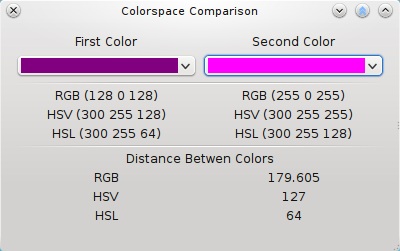
\includegraphics[width=0.5\textwidth]{colorspace_comparison_application.png}
  \end{center}
  \caption{Colorspace comparisons between a light purple and a dark purple. HSL has the advantage here, correctly indicating that these colors are similar.}
  \label{fig:colorspaceComparison}
\end{figure}

{%
\newcommand{\mc}[3]{\multicolumn{#1}{#2}{#3}}
\definecolor{lightBlue}{rgb}{0,0,1}
\definecolor{darkBlue}{rgb}{0,0,0.501961}
\definecolor{darkRed}{rgb}{0.501961,0,0}
\definecolor{lightRed}{rgb}{1,0,0}
\definecolor{black}{rgb}{0,0,0}
\definecolor{lightGreen}{rgb}{0,1,0}
\definecolor{lightYellow}{rgb}{1,1,0}
\begin{table*}
\begin{center}
\begin{tabular}{ccccc}
% use packages: color,colortbl
First Color & Second Color & RGB Dist & HSV Dist & HSL Dist\\
\mc{1}{>{\columncolor{lightBlue}}c}{×} & \mc{1}{>{\columncolor{darkBlue}}c}{×} & 127 & 127 & 64\\
\mc{1}{>{\columncolor{darkRed}}c}{×} & \mc{1}{>{\columncolor{darkBlue}}c}{×} & 181 & 240 & 240\\
\mc{1}{>{\columncolor{lightRed}}c}{×} & \mc{1}{>{\columncolor{darkBlue}}c}{×} & 285 & 272 & 248\\
× & \mc{1}{>{\columncolor{black}}c}{×} & 441 & 255 & 255\\
\mc{1}{>{\columncolor{lightGreen}}c}{×} & \mc{1}{>{\columncolor{lightYellow}}c}{×} & 255 & 60 & 60\\
\mc{1}{>{\columncolor{black}}c}{×} & \mc{1}{>{\columncolor{darkBlue}}c}{×} & 128 & 373 & 357
\end{tabular}
\end{center}
\caption{Some examples of colors and their respective distances in the three colorspace models. R, G, B, S, V, L all vary between [0, 255]. Hue varies between [0, 360]. {\bf I`m not so sure about this wording.. thoughts? } `Good' values are subjective, based on the authors' ideas on what colors are likely to be part of the same object in an image seen by the computer or robot.}
\end{table*}
}%



\subsection{Distance Calculation}

%We want to place emphasis on distance. Two colors with zero difference in color space but high dist in euclidean space were being categorized as the same object. Want to make them different. Could try to find an image (4 pieces of paper?) that regular x,y dist fails but 1.5*x,y works.

Since the GNG treats each of the five inputs equally, sometimes vectors separated by a large distance but with very similar colors end up having a small distance in object space and so the two vertices end up categorized as part of the same object. There are three color inputs and only two distance inputs, so the color information can be overpowering. To fix this problem we added emphasis to the $xy$ distance metric by adding an additional $1.5 * xyDistance$ to the total object distance metric. Thus, the formula is as follows:
\begin{align*}
  distance = &\sqrt{(x_2-x_1)^2+(y_2-y_1)^2+(h_2-h_1)^2+(s_2-s_1)^2+(l_2-l_1)^2} \\ &+ 1.5*\sqrt{(x_2-x_1)^2+(y_2-y_1)^2}
\end{align*}

In Figure \ref{fig:distModification} we see a clear effect of the distance modifications. When the additional $xy$ distance is not taken into account, the two sheets of blue paper remain undifferentiated after 10,000 steps. Once we make the modification, the GNG quickly identifies the sheets.

\begin{figure}[h!]
  \centering

  \subfigure[Categorization without distance modification.]{
    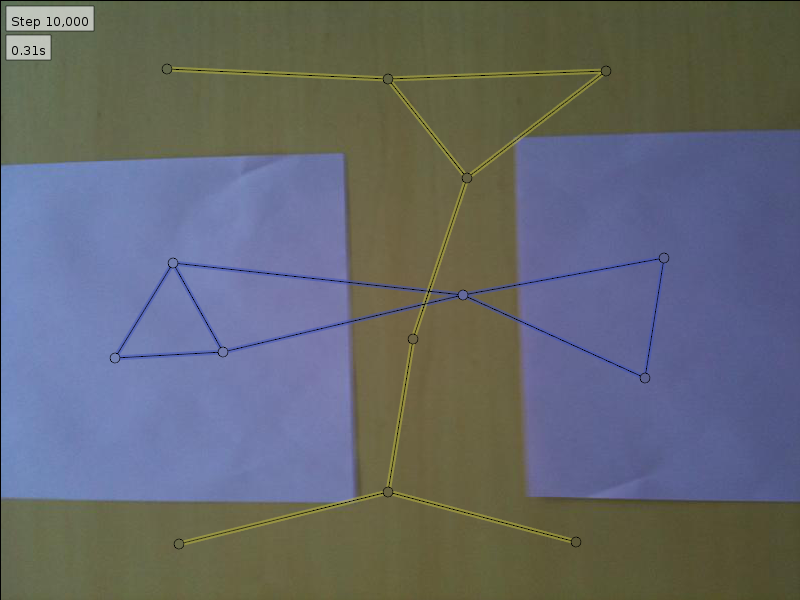
\includegraphics[width=0.45\textwidth]{paper2_nodist_modification.png}
  }
  \subfigure[Categorization with distance modification.]{
    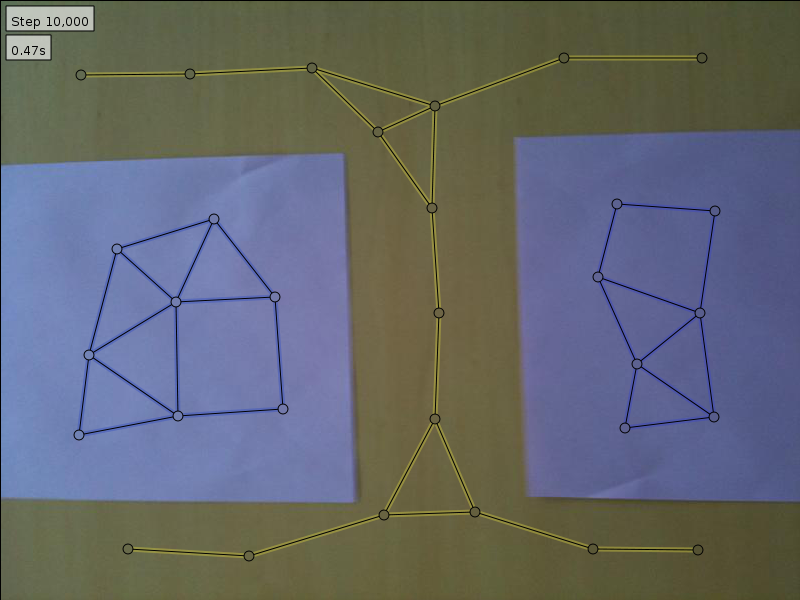
\includegraphics[width=0.45\textwidth]{paper2.png}
  }

  \caption{GNG categorizing 2 sheets of paper with and without the distance modification.}
  \label{fig:distModification}
\end{figure}

\subsection{gngviewer}

Because of the incremental nature of our modifications to the GNG we needed a solid way of visualizing the results of the GNG. From this need the gngviewer emerged. The viewer is domain-specific, it assumes a GNG with inputs that contain pixel information. The viewer runs asynchronously from the GNG and provides a continuously updating view of how the GNG is changing. It provides layers that show the nodes along with their color information, the edges and the subgraphs that have been generated.


\section{Modifications to Growing Neural Gas}
\label{sec:modificationsGNG}

%\subsection{Aging Growing Neural Gas (AGiNG)} --> Ask Stromme, is it okay to remove this and just have subsections (instead of subsubsections) below

We have identified a few limitations with the original Growing Neural Gas algorithm. Most of these limitations are exposed when the input image data changes over time. These important considerations for our problem domain and it is important to address these. Each will be discussed separately along with the modifications to the core GNG that resolve or alleviate the issue at hand. The sum of these small changes significantly changes how the GNG adds and removes nodes and edges and how it categorizes its input space. We introduce our new type of GNG outfitted with these changes as AGiNG. AGiNG is designed to provide the standard GNG with information regarding the history of nodes and edges. It is composed of a number of small modifications which will be discussed individually in subsequent sections.

\subsection{Node Insertions - Periodic and Error Dependent}

The first addition to the GNG dealt with node insertion. The original GNG inserted nodes on a fixed interval. This caused a few complications. Firstly, it didn't allow the GNG to come to any sort of natural equilibrium. The longer the GNG was run the more nodes there would be. This is a problem because we are running the GNG continuously for many thousands of time steps. In \citeA{lee} this issue is addressed by only adding new nodes when the average error is above some error threshold. This helps but still causes problems for our particular inputs. Because the inputs that we give to the GNG can be so dissimilar the average error can be extremely high even if hundreds of new nodes are added. To lower the error it is necessary to run the GNG for a number of time steps to allow the nodes to spread out and start categorizing the input space. To allow for this we have combined the two GNG node insertion policies. New nodes are added at most every n time steps (where n is normally around 100) but only while the average error is greater than a thresholded value (normally between 0.1 and 0.01). This allows a natural equilibrium to occur, where the GNG adds more nodes when the scene becomes more difficult to categorize.

\subsection{Normal Edge Age - Edge Removal}

Growing Neural Gas has a built in sense of edge ages. Each iteration, all of the edges that are connected to the selected `winner' node are incremented in age. The age of an edge is reset when it is the edge between the primary and secondary winner for any given iteration. Edges are removed when they exceed some threshold age. This normal edge age does well with what it was originally designed to do: remove edges when they are not between similar enough nodes, where similar is defined as distance relative to the distance of other nodes.

\subsection{Total Edge Age - Discounting Edges}

An edge with a normal edge age of 0 could mean one of three things. Either the edge was just added or it was just reset or it was added at some time in the past and then was never connected to a winning node and thus was never updated. This is very ambiguous and therefore normal edge age isn't adequate for our needs. We started by defining a sense of total edge age. This is an integer counter which is incremented for each edge every single time step. If an edge is added or re-added its total age starts at 0. This allows us to differentiate between the first and second options. If the edge has been around for a long time and has been constantly updated then its total age will be high. However, if the edge was just added then its edge age will be low. We use this information to discount edges when subgraphs are generated for the object detection and tracking. Young ages are not counted when the subgraph generator traverses graphs to generate objects. The reasoning for this is that old edges have a much better chance of representing a strong connection internal to an object where young edges are likely to be temporary connections made by choosing some noisy input point. 

In Figure \ref{fig:totalEdgeAge} we have an image where we would ideally identify three distinct objects. While the GNG has created one single graph where every node is technically reachable from every other node. Since we are discounting any node with total edge age less than 2000 steps (indicated by the pop-ups next to the young edges) we see three disjoint subgraphs. Each of the edges connecting one subgraph to another are young enough that they are discounted. Thus, even when the GNG does not perfectly fit the input space, we can use the total age to get an extra level of context and provide a buffer against misclassifying the scene.

\begin{figure}[h!]
  \centering
    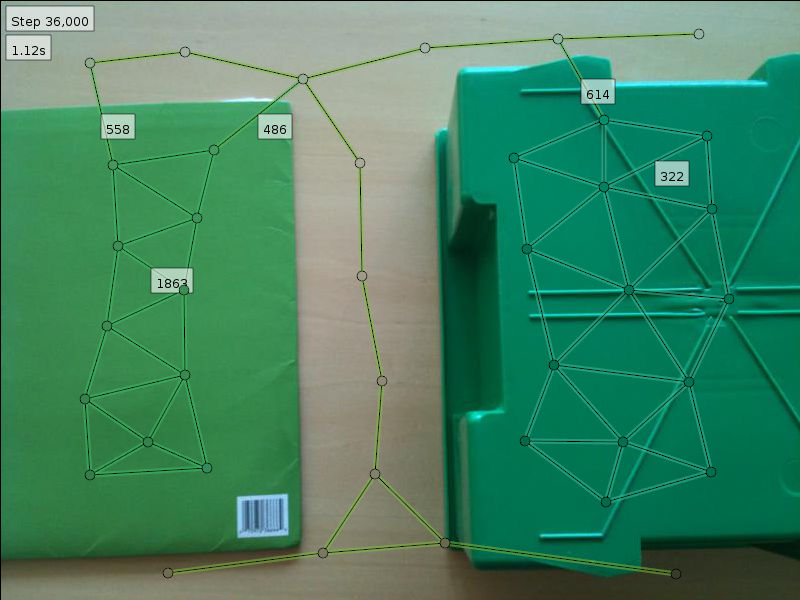
\includegraphics[width=0.5\textwidth]{total_edge_age.png}

  \caption{Two green objects separated by a small distance. Numbers next to younger edges indicate their current total age. To keep the display uncluttered, edges with age over 2000 steps are not annotated. Since edges with total age $< 2000$ are discounted, we have three effectively disjoint subgraphs, identifying the folder, box, and table background.} 
  \label{fig:totalEdgeAge}
\end{figure}

\subsection{Edge Last Updated - Removing old Edges}

Even with total edge age it is ambiguous how long an edge has been around for in terms of physical time. This is important once images begin to be dynamic instead of static. If a webcam is providing 30 frames per second then an edge that was added 5 seconds ago isn't useful if it hasn't been updated. In this case even the total edge age can't provide the necessary information. There is the possibility that it was an edge that had lasted for a long time and thus had an old total age but then the scene switched quickly (lights were turned on, something fell in front of the camera) and the nodes that the edge was connected to were no longer updated. This caused the appearance of `ghost structures' that were left behind when the scene changed. To account for this a last updated parameter was added to the each edge. The GNG itself keeps track of how many seconds it has been since it was started. Each time an edge is modified it resets its last updated parameter to the current runtime of the GNG. Each time step the GNG checks for ages that haven't been updated in a set amount of time (usually around 5 seconds) and begins to remove them one at a time. {\bf TODO: Before/After pictures with ghost structures.}

\subsection{Edge History}

One other value to track that is implemented in Aging but is currently not used for anything is a sense of edge history. This provides a per-edge counter that is incremented every time step when an edge is present between two nodes. If an edge is present for a while, then is removed but is subsequently re-added the counter remains intact. This is implemented using a hash table, hashing on the unique ids of the two nodes that the edge connects. A possible future use for this counter is to give a sense of how close nodes were throughout the history of the GNG. If nodes were close to each other there is a good chance that an edge would exist between them and thus the edge history would be high. This could be useful for objects that split apart and later reform.

\subsection{Color Barrier Across Object Boundaries}

%If color difference is too great between two nodes, don't add an edge. Since we describe objects in terms of their color, makes sense.
Even with the modifications described above, experiments showed that the GNG was still adding an large number of edges between nodes that were right along the boundary edges of objects. For example, if the GNG were categorizing a scene with a black wallet against an off-white wall, a node from the foreground and from the background would often be connected since they were very close in distance. To solve this problem, a check was put in place each time an edge was to be added or the age of an existing edge was to be reset. The hues of the nodes are compared, and if their difference is greater than a specified value the edges are not created. Through experimentation we found that a good threshold value is 0.1, which corresponds to a 36 point difference in the 360-degree hue space. As a rough heuristic, this is about half way between any two consecutive bands of the color strip ({\bf reference color strip below? put this section below Methods?})

After implementing this change, we quickly saw our graph dwindle down to a size of zero. Since the early stages of the GNG consist of creating nodes between spaces that almost always differ in hue values greater than the threshold, very few or no nodes were being created. We resolved that this processing step had to be applied only once the GNG was more developed. This led to the additional check of average error against the target error. If average error is above target error, nodes are no longer being added to the graph, so it is safe to either disallow connections or the resetting of age (which can lead to an edge's removal). With this additional condition, results improved markedly. Edges between objects were much better defined and subgraphs representing each object were more likely to remain disjoint.

In Figure \ref{fig:colorBarrier} below, we see the GNG categorizing three sheets of purple paper on a tan background. On the left, the color barrier is not enabled. We see that connections between the lower-left sheet of paper, the top sheet, and the background all exist when they should not. Contrast this with the right image where the color barrier is enabled. There are clear distinctions between the subgraphs with no inappropriate edges.

\begin{figure}[h!]
  \centering

  \subfigure[Categorization without color barrier.]{
    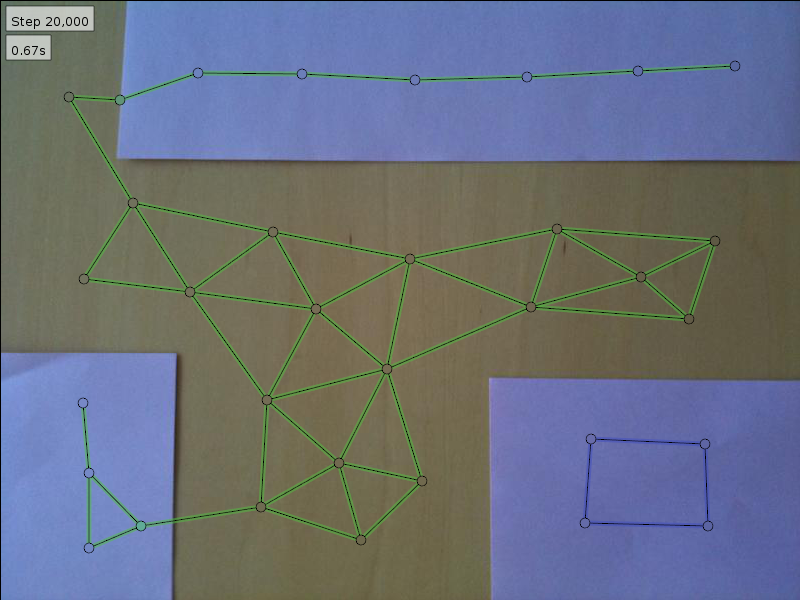
\includegraphics[width=0.45\textwidth]{paper3_nocolorbarrier.png}
  }
  \subfigure[Categorization with color barrier.]{
    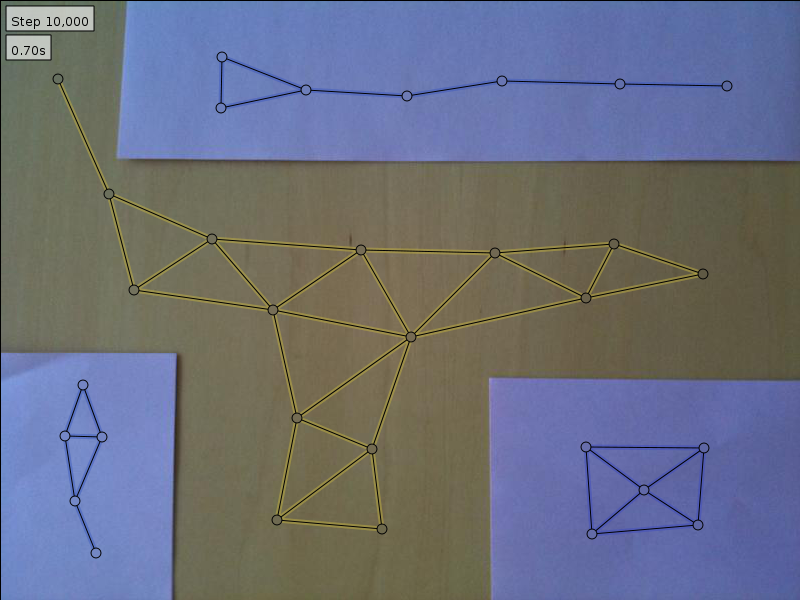
\includegraphics[width=0.45\textwidth]{paper3.png}
  }

  \caption{GNG categorizing 3 sheets of paper with and without the color barrier. Status is shown after 20,000 steps in Figure (a), 10,000 in Figure (b).}
  \label{fig:colorBarrier}
\end{figure}

\section{Object Tracking}
\label{sec:objectTracking}

%How we define objects -- subgraphs
Once the GNG has built up a graph representing the object space, we want to automatically identify and track objects in the scene. We can define objects in the graph in terms of subgraphs. Since we are relying on distance and color as markers of objects and are feeding that information into the Growing Neural Gas, over time the graph will partition itself into smaller, disjoint subgraphs representing objects in the scene. Thus each subgraph represents a single object that we can identify and track.

\subsection{Subgraph Generation}

In order to eventually track objects we must first identify them. Thus we need to have a method of finding the disjoint subgraphs that constitute our objects. The algorithm that accomplishes this is a layer on top of breadth-first search. It starts by picking a random vertex in the graph and looking at which vertices are reachable from it. Once no more vertices are reachable from the initial selection, we check if any vertices remain unvisited and, if so, repeat the process. The algorithm is described as pseudocode in Algorithm \ref{alg:detectingSubgraphs}.

\begin{Algorithm}[h!]
\begin{program}
  |create empty list of subgraphs, | subgraphList \rcomment{(Will contain all subgraphs)}
  \WHILE |graph contains unvisited nodes|:
    V = | an unvisited vertex in graph|
    |add | V | to queue, | q
    |create empty list, | subgraph \rcomment{(Keeps track of current disjoint subgraph)}
    \WHILE q | is not empty|:
      search = |takeFirstElement in | q \rcomment{(Removes and returns first element)}
      |mark | search | as visited|
      |add | search | to | subgraph
      |add neighbors of | search | to | q \untab
  |add | subgraph | to | subgraphList
\end{program}
\caption{Pseudocode for Detecting Subgraphs}
\label{alg:detectingSubgraphs}
\end{Algorithm}

We note that this algorithm is efficient and fast enough so that we can run it every time we update the visualizer without slowdown. We store the unvisited nodes in a hash table for constant time access and removal at some cost to space. The runtime of the algorithm is $O(\|V\|+\|E\|)$ with $\|V\|$ vertices and $\|E\|$ edges. The space requirement is $O(\|V\|+\|E\|+\|G\|)$ for the graph $G$. Since the size of graph generated by the GNG is rarely more than a hundred nodes, time and space requirements are very reasonable.

\subsection{Tracking Subgraphs}

%Pick an exemplar, track exemplar by counting number of intersecting nodes. Pseudo Code
Once we have a set of subgraphs that details the objects the GNG has identified, we need a way of tracking them. As an object moves through the scene, the associated subgraph will also translate to best fit the new object space. Some nodes will be added to fill the space while others which are no longer useful will be deleted. But in general the subgraph associated with an object at time $t_0$ will share most of the nodes as the subgraph associated with the same object at $t_1$. We can formalize this intuitive notion of subgraph tracking by choosing an exemplar subgraph at $t_0$ to track. Then, at $t_1$, we recompute the subgraphs and compare each new subgraph to the exemplar. Whichever subgraph shares the most points with the exemplar becomes the new exemplar. The algorithm is again described as pseudocode in Algorithm \ref{alg:trackingSubgraphs}.

\begin{Algorithm}[h!]
\begin{program}
  |choose an exemplar if one has not been chosen|
  maxCount = 0
  \FOR currentSubgraph \IN subgraphList: \rcomment{($subgraphList$ from subgraph generation})
    count = 0
    \FOR node \IN currentSubgraph:
      \IF node | is in | exemplar:
        count|++| \untab \untab
    \IF count > maxCount:
      maxCount = count
      exemplar = currentSubgraph
\end{program}
\caption{Pseudocode for Tracking Subgraphs}
\label{alg:trackingSubgraphs}
\end{Algorithm}

We can again look at the runtime and space requirements for the algorithm. We need to traverse every node in the graph and then check if that node is in the exemplar. Thus this has a runtime of $O(\|G\|*\|exemplar\|)$. In the worst case this is $O(\|G\|^2)$ if the exemplar is the entire graph, $G$. In every realistic case, however, the exemplar will be markedly smaller than the approximately one hundred node graph. The algorithm requires $O(\|G\|+\|exemplar\|)$ space.

\section{Experiments}
\label{sec:experiments}

%Talk about broad classes of experiments -- static, moving, and AIBO

There are two broad categories of experiments we conducted. The first distinguished between static and moving images. Static images were used as an early benchmark for testing whether or not our algorithm could correctly categorize an image given unlimited time. Moving images tested the ability of the GNG to both adapt to new situations after creating an initial categorization scheme and to do so in real time. The second category of experiments consisted of either computer-generated images or real-life pictures taken with a camera or captured with a webcam. 

In general, we found that computer-generated images (both static and moving) were very easy for the GNG to categorize. Real-life examples contain many more details and are much noisier. In the sections below we detail our experiences with various object detection and tracking tasks. We also experimented with a Sony AIBO reacting appropriately to objects identified by the Growing Neural Gas. Finally we discuss some of the limitations of our algorithm illuminated by these experiments.

\subsection{Static Images}

% Easy. Real and Computer-generated

The key aspect of static images is the categorization task the GNG is tackling is not time sensitive. Thus these tests were a great tool to incrementally check whether or not our GNG was on the right path towards correctly identifying objects in the scene. Figure \ref{fig:rgbStatic} depicts a simple image generating using GIMP\footnote{The GNU Image Manipulation Program, \url{http://www.gimp.org}} with three colored blocks (red, green, and blue) on a white background. We see that four disjoint subgraphs have formed, one for each object and another for the background. These subgraphs form very quickly (10,000 cycles or less than one second) and stay disjoint over time. 

\begin{figure}[h!]
  \begin{center}
    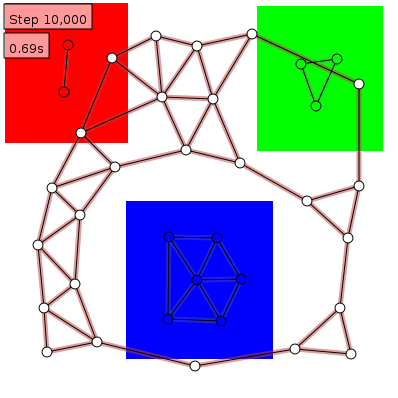
\includegraphics[width=0.5\textwidth]{rgb_static.png}
  \end{center}
  \caption{Computer-generated static image with red, green, and blue blocks on a white background. GNG quickly and correctly categorizes image.}
  \label{fig:rgbStatic}
\end{figure}

The pictures below (Figure \ref{fig:1-4papers}) contain the GNG trying to categorize one, two, three, and four sheets of purple paper on a tan table background. As we see, with the GNG set on reasonable default settings ({\bf see Apendix \ref{appendix:staticImgParams}}), the first three images are categorized very accurately. Indeed, the GNG very quickly distinguishes between background and foreground images and correctly identifies distinct sheets of paper. 

\begin{figure}[h!]
  \centering

  \subfigure[Categorization on one sheet.]{
    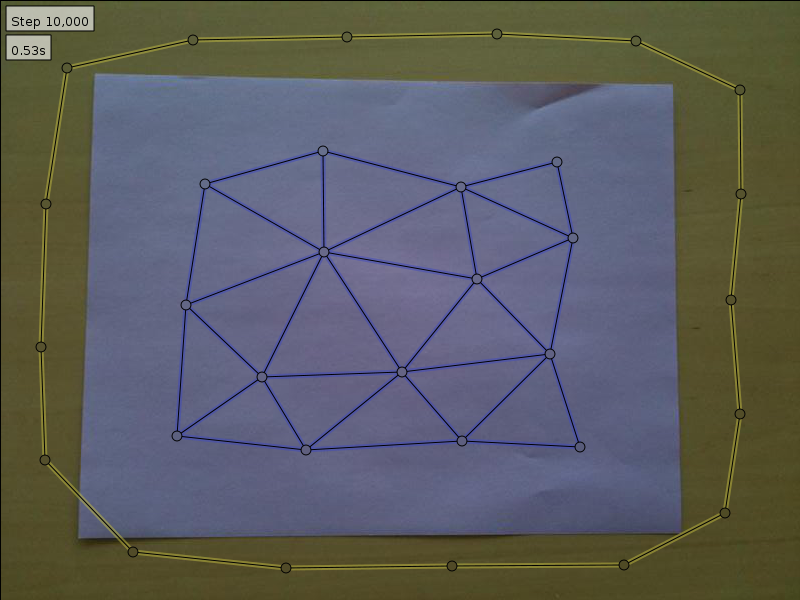
\includegraphics[width=0.45\textwidth]{paper1.png}
  }
  \subfigure[Categorization on two sheets.]{
    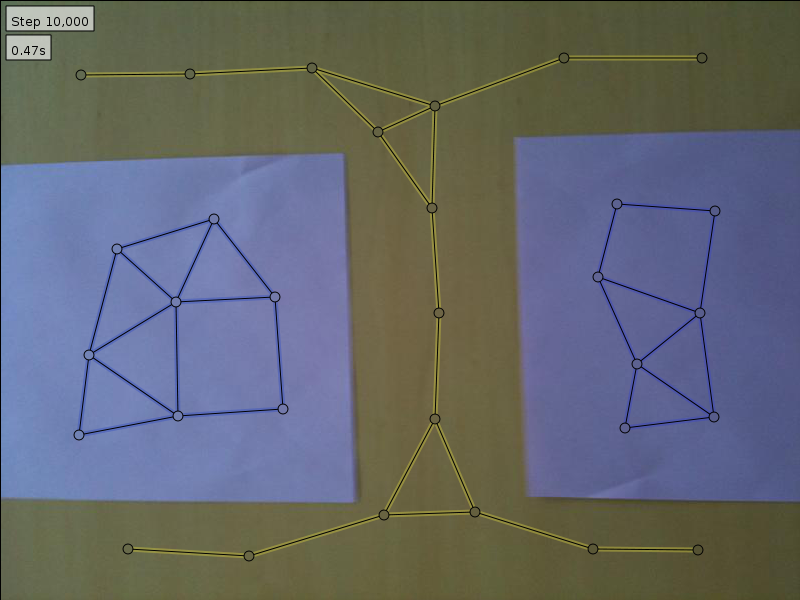
\includegraphics[width=0.45\textwidth]{paper2.png}
  }
  \subfigure[Categorization on three sheets.]{
    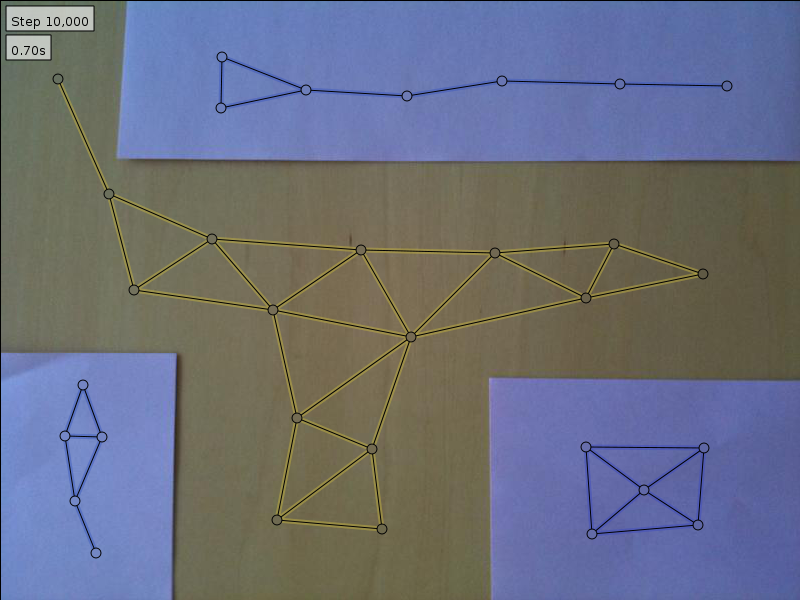
\includegraphics[width=0.45\textwidth]{paper3.png}
  }
  \subfigure[Categorization on four sheets.]{
    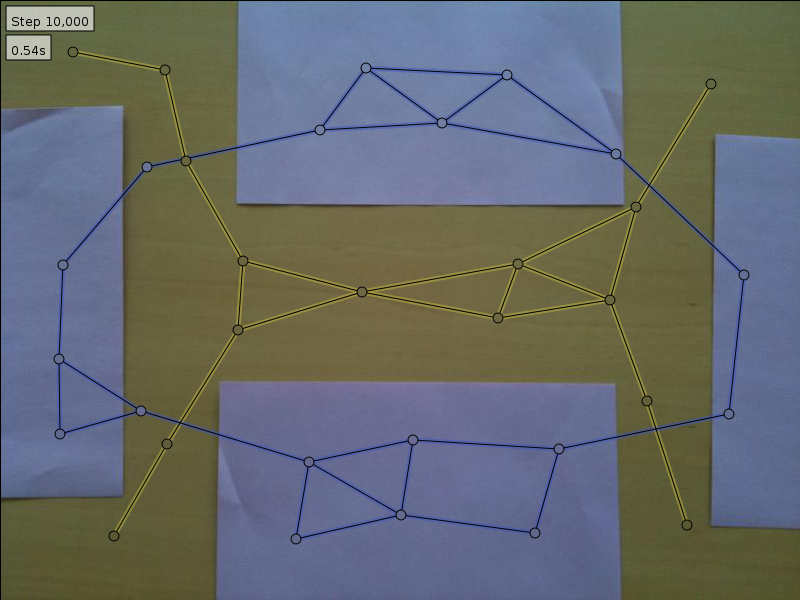
\includegraphics[width=0.45\textwidth]{paper4.png}
  }

  \caption{GNG categorizing sheets of purple paper on a table.}
  \label{fig:1-4papers}
\end{figure}

The final image with four sheets, however, is not correctly categorized. The GNG contains only two disjoint subgraphs instead of five. The table is correctly identified, but all four sheets of paper are part of the same subgraph. We show the result after 10,000 iterations, but given any number of iterations the graph's basic structure does not change. This is the result of the target error being too high so the GNG does not need add more nodes to better fit the object space. We expect that lowering the target error will cause the GNG to create more nodes and better categorize the space. In \ref{fig:paper4Lowerror} we lower the target error from 0.05~to~0.01 and we see a marked improvement. The image in Figure \ref{fig:paper4_10,000} the represents the GNG after 10,000 iterations (the same number of iterations as before). We see the GNG is beginning to create disjoint subgraphs but has not yet accurately categorized the object space. After 20,000 iterations (Figure \ref{fig:paper4_20,000}), however, the GNG has fully and correctly broken the image up into five distinct subgraphs that we can track. Thus, by lowering the target error we can more accurately describe a space, but it comes with a time cost. 

\begin{figure}[h!]
  \centering
  \subfigure[Categorization after 10,000 steps.]{
    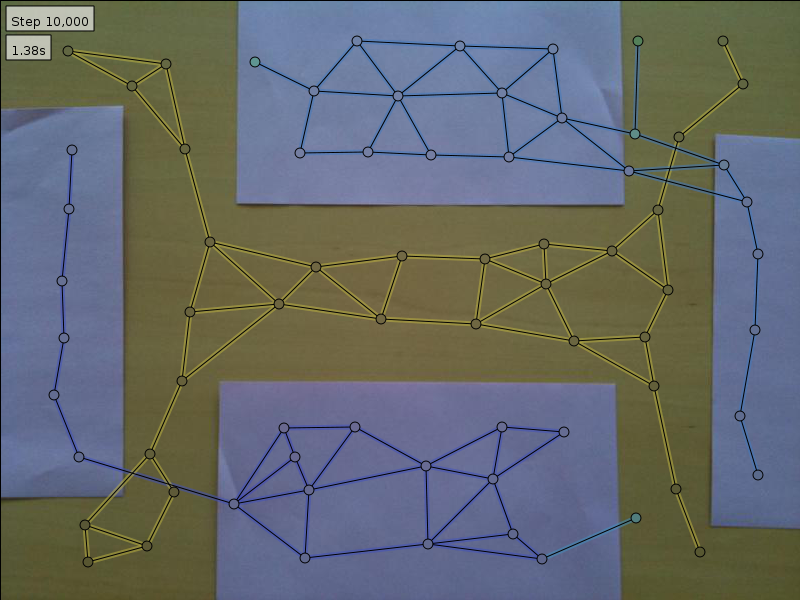
\includegraphics[width=0.45\textwidth]{paper4_lowerror10000steps.png}
    \label{fig:paper4_10,000}
  }
  \subfigure[Categorization after 20,0000 steps.]{
    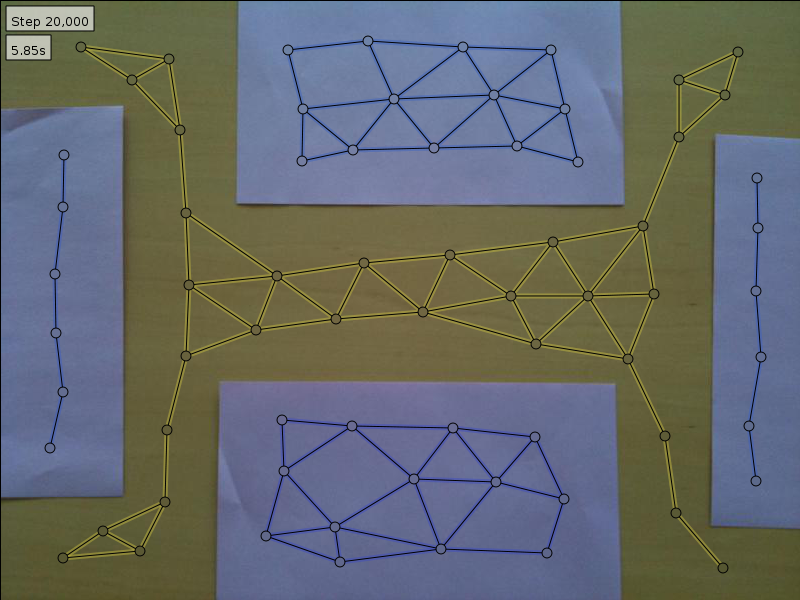
\includegraphics[width=0.45\textwidth]{paper4_lowerror20000steps.png}
    \label{fig:paper4_20,000}
  }

  \caption{GNG correctly categorizing four sheets of paper with adjusted error.}
  \label{fig:paper4Lowerror}
\end{figure}

\subsection{Moving Images}

%GNG is able to follow what's going on. Very cool!
We have also experimented with tracking objects in moving images. Here we again consider computer-generated sequences of images and real-life video, taken from a webcam. In Figure \ref{fig:rgbMoving} we see the familiar image with red, green, and blue blocks on a white background. This time, however, the red block moves towards the center of the scene and then outward back to its original position. The GNG is able to quickly categorize the red block and then follow it as it travels around the scene. Note also that in addition to the green and blue blocks having stable categorizations throughout the experiment, the white background nodes moved out of the way as the red block moved. This is encouraging, showing that the GNG is able to adapt over time.

\begin{figure}[h!]
  \centering
  
  \subfigure[Red block in upper left corner.]{
    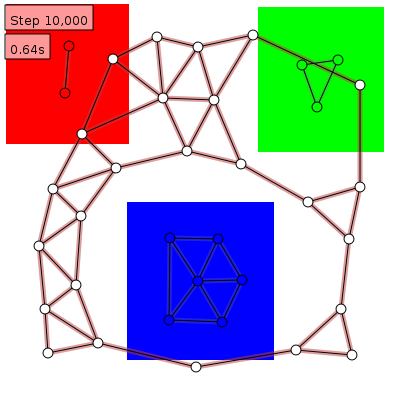
\includegraphics[width=0.45\textwidth]{rgb_motion1.png}
  }
  \subfigure[Red block moving towards center.]{
    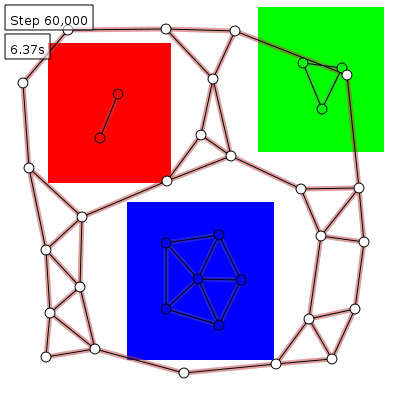
\includegraphics[width=0.45\textwidth]{rgb_motion2.png}
  }
  \subfigure[Red block at center of scene.]{
    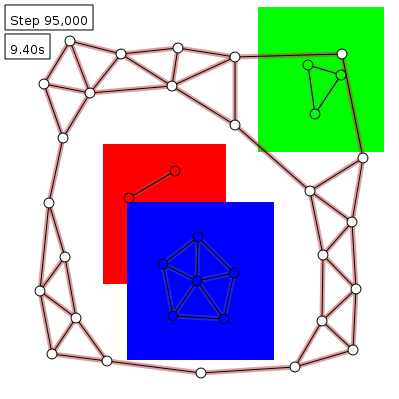
\includegraphics[width=0.45\textwidth]{rgb_motion3.png}
  }
  \subfigure[Red block returning to upper left corner.]{
    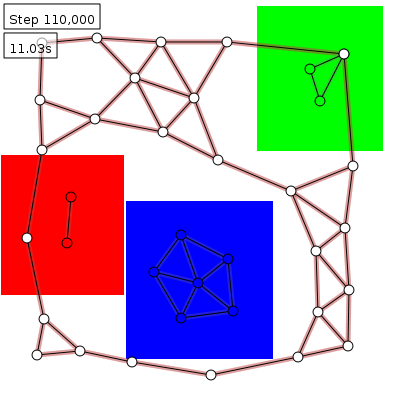
\includegraphics[width=0.45\textwidth]{rgb_motion4.png}
  }
  
  \caption{GNG categorizing a red block moving through a scene.}
  \label{fig:rgbMoving}
\end{figure}

A webcam was also used to see how the GNG dealt with real-time updates from noisy data. Results here were less successful that in past trials but still very encouraging. When presented with clear foreground objects and a distinct background, the GNG was able to correctly classify various foreground objects. On the other hand, complex scenes like faces or full room views were very difficult for the GNG to categorize. In Figure \ref{fig:webcam} we placed an arm wrapped in a black cloth in front of a whiteboard with carefully controlled lightening. The GNG was able to quickly (within three seconds) identify the basic shape of the arm but it took a full ten seconds before clear and distinct subgraphs between background and foreground emerged. As with the colored blocks above, as the arm moves through the scene the background categorization moves out of the way to make space.

\begin{figure}[h!]
  \centering
  
  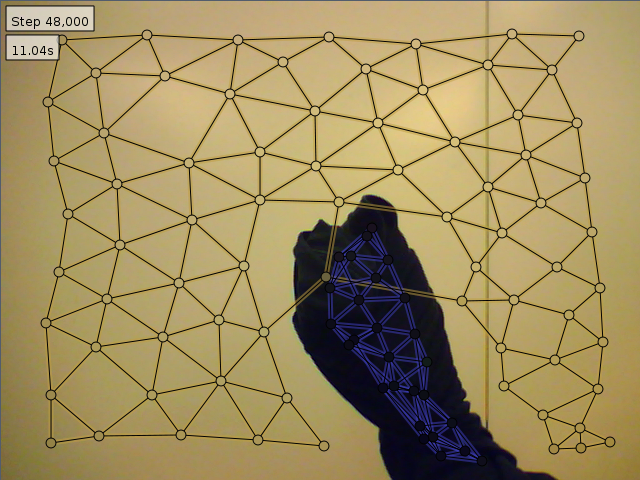
\includegraphics[width=0.45\textwidth]{webcam.png}
  
  \caption{GNG categorizing a webcam image.}
  \label{fig:webcam}
\end{figure}

\subsection{Real-Time Object Tracking with AIBO}

% Here's where the implicit memory really helps. As objects move and disappear, GNG is able to cull useless errors.
We were able to interface with the AIBO using libraries we created in C++ to make the robot turn its head appropriately as an image being tracked moves around the scene. Initially we tried using the ABIO's built-in camera but grabbing images over the wireless connection kept the semaphore locked for too long and thus caused the gngviewer to update slowly and irregularly. This made experimentation very difficult using only tools available to the AIBO. As a proof of concept, to show our GNG could correctly track objects, we instead used the webcam and pretended it was the AIBO's camera. That is, when an object moved to the left of the scene, we caused the AIBO to turn its head to the left. When an object moved back to the center, the AIBO returned its head to the forward position.

Our experiment consisted of a black wallet on a white background. The wallet would be selected as the object to follow by the following process. We specified that we wanted to follow {\em some} black object. Once the subgraphs had been generated, the subgraph with the average color closest to black was chosen as the object to follow. As the subgraphs change, the designated follow subgraph changes with it. At any time we can query the ``center'' of the subgraph, which calculates the average of all the $(x,y)$ points in the subgraph. We can use this average to figure out which of six quadrants the object is currently in. There are left, middle, and right sections and each of those can be broken into top and bottom sections. Provided the object was not moved too quickly, we were able to successfully ``track'' the object by making the AIBO's head turn appropriately. When the follow object moved too quickly, many nodes that used to be part of the object moved into the background and we switched to following the background, which isn't very useful. We discuss this in more depth in section \ref{sec:future}.

\subsection{Limitations}

%No sense of edges or depth, so we perform poorly on complex, busy images. Example of busy image? Computer in Stromme's room?
Our modified implementation of Growing Neural Gas is not without its limitations. While we are encouraged that our system can do as well as it does without any edge detection, we recognize that edge recognition is a very natural and effective way to identify objects. Additionally, we are not providing any depth information to our categorization machine. As such, the GNG does very poorly on very complicated objects. For example, in Figure \ref{fig:badCategorization} we see an image of a computer on a desk with a host of other objects and strange lighting effects. The categorization simply fails. Some nodes appear to be clustered in areas of importance like the laptop and the background, but no disjoint subgraphs appear and no context can really be gained from the categorization. Thus, while we have some promising results, we must acknowledge that there is much work to be done.

\begin{figure}[h!]
  \centering
  
  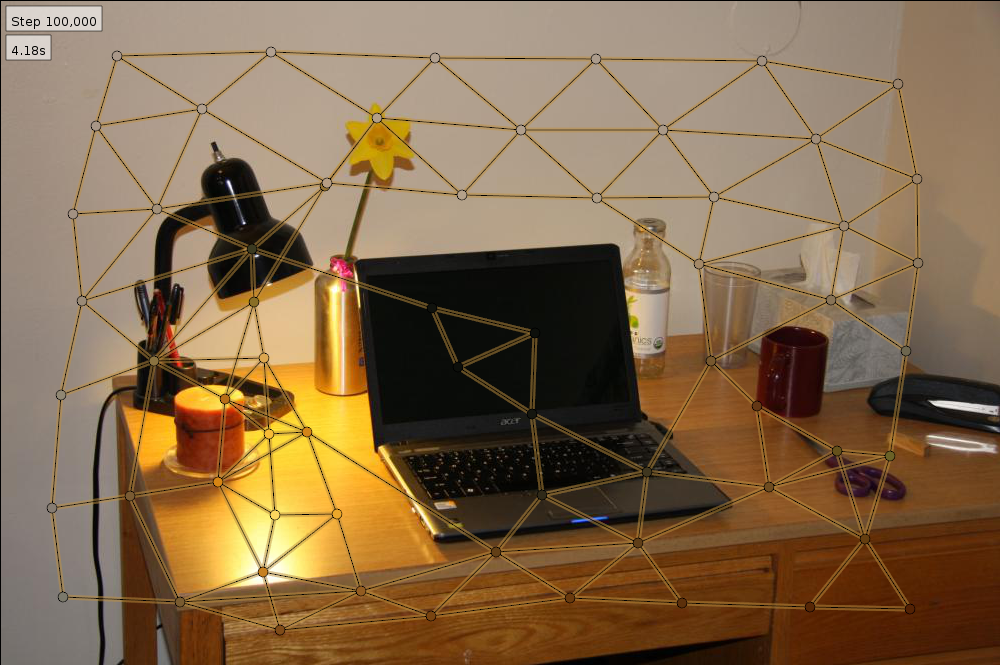
\includegraphics[width=0.45\textwidth]{bad_categorization.png}
  
  \caption{GNG trying (in futility) to categorize a complex image.}
  \label{fig:badCategorization}
\end{figure}

\section{Discussion}
\label{sec:discussion}

We have introduced an extension of the GNG algorithm, the Aging Growing Neural Gas (AGiNG), specifically aimed at  object detection and tracking. We can identify objects by sending color and distance information as input, keeping a close eye on two types of edge age, and using domain-specific knowledge to cull edges or disallow their creation. Our graph thus represents distinct objects represented as disjoint subgraphs. We can use efficient traversal algorithms to identify and track these subgraphs as objects move through the scene. We have described the changes we made to the original algorithm and have shown the effects of our modifications. Finally, we have detailed experiments showing where the AGiNG performed well and where there is room for improvement. Importantly, we have shown that one does not necessarily need to rely on edge detection heuristics to accurately identify objects. Using just color and distance information, we can accurately classify and track objects as they move through a scene.

\section{Future Work}
\label{sec:future}

We realize that we are giving the GNG an enormous amount of input points. In a 1000x1000 pixel image, similar in size to the ones that were used in this paper, the GNG would have to perform one million iterations to visit every pixel. This is obviously not happening with 10000 iterations. Inputs are selected randomly which should help the GNG in classifying the entire image instead of just parts of it but because it is random there is a chance that it will not provide critical points as input vectors. One way to help this might be to simplify the images, reducing their resolution. A 100x100 pixel image can have much of the same large-scale detail and only requires ten thousand iterations to fully visit. This is much more within the realm of the speeds seen using the C++ implementation of libgng shown in this paper.

The GNG was also seen to be very sensitive to changes in the distance function between two points. The different parts of color and distance need to be weighted properly to get valid results. One thought was to reduce the color information to a grayscale image. This would reduce the number of color inputs from 3 to 1, which would bring down the total number of inputs to the GNG down to only 3 (x, y, grayscale). This would intrinsically weight the physical distance more than the color distance and might render the artificially increased physical distance unnecessary. It might also allow us to run the GNG with a smaller error threshold and still perform the same number of iterations because fewer computations are needed. As shown in Figure \ref{fig:paper4Lowerror} a smaller error threshold allows the GNG to detect and classify smaller objects.

Currently our work with the AIBO has been a proof of concept. When using a webcam connected to the computer running the GNG we can turn the AIBO's head to the left or right, up or down as the objects it's ``following'' moves around in the webcam image. When testing with the AIBO's internal camera, the wireless connection was too slow to get real-time updates. Moving forward, we want to make the data transfer between the AIBO and GNG smoother so that lag is minimized. Once we have a better pipeline in place, we can expand the actions available to the AIBO. As an object moves across a scene we would expect the AIBO to move not just its head but its entire body to track the object. For example if the object is in the upper left quadrant of the scene, the AIBO should rotate to the left until the object is centered and then should tilt its head upwards. We are hopeful for the future given our progress thus far, but we acknowledge there is much to be done.

\bibliographystyle{apacite}
\bibliography{references}

\appendix
\section{Default Parameters for Static Images}
\label{appendix:staticImgParams}

Here we present the default values that we use when running the GNG. Assume these values if not otherwise specified. We continue inserting nodes until the average error has reached the \verb+targetError+ threshold. The \verb+winnerLearnRate+ is used to adjust the closest unit towards the input point. We use the \verb+neighborLearnRate+ to adjust the other neighbors towards the input point. Edges older than the \verb+maxEdgeAge+ are removed. All errors are reduced by \verb+errorReduction+ at each step. A new unit's error is reduced by \verb+insertErrorReduction+. We add a \verb+delay+ millisecond delay to each step. The minimum number of steps before inserting a new node is \verb+nodeInsertionDelay+. Edges are not created if the color difference between nodes is above the \verb+maxEdgeColorDiff+. Finally, we run \verb+totalIterations+ iterations before stopping.

\begin{verbatim}
targetError = 0.05
winnerLearnRate = 0.05
neighborLearnRate = 0.01
maxEdgeAge = 50
errorReduction = 0.05
delay = 0
totalIterations = 10000
\end{verbatim}

\end{document}
